\chapter{Introduction}
\label{chap:intro}

\begin{figure}
    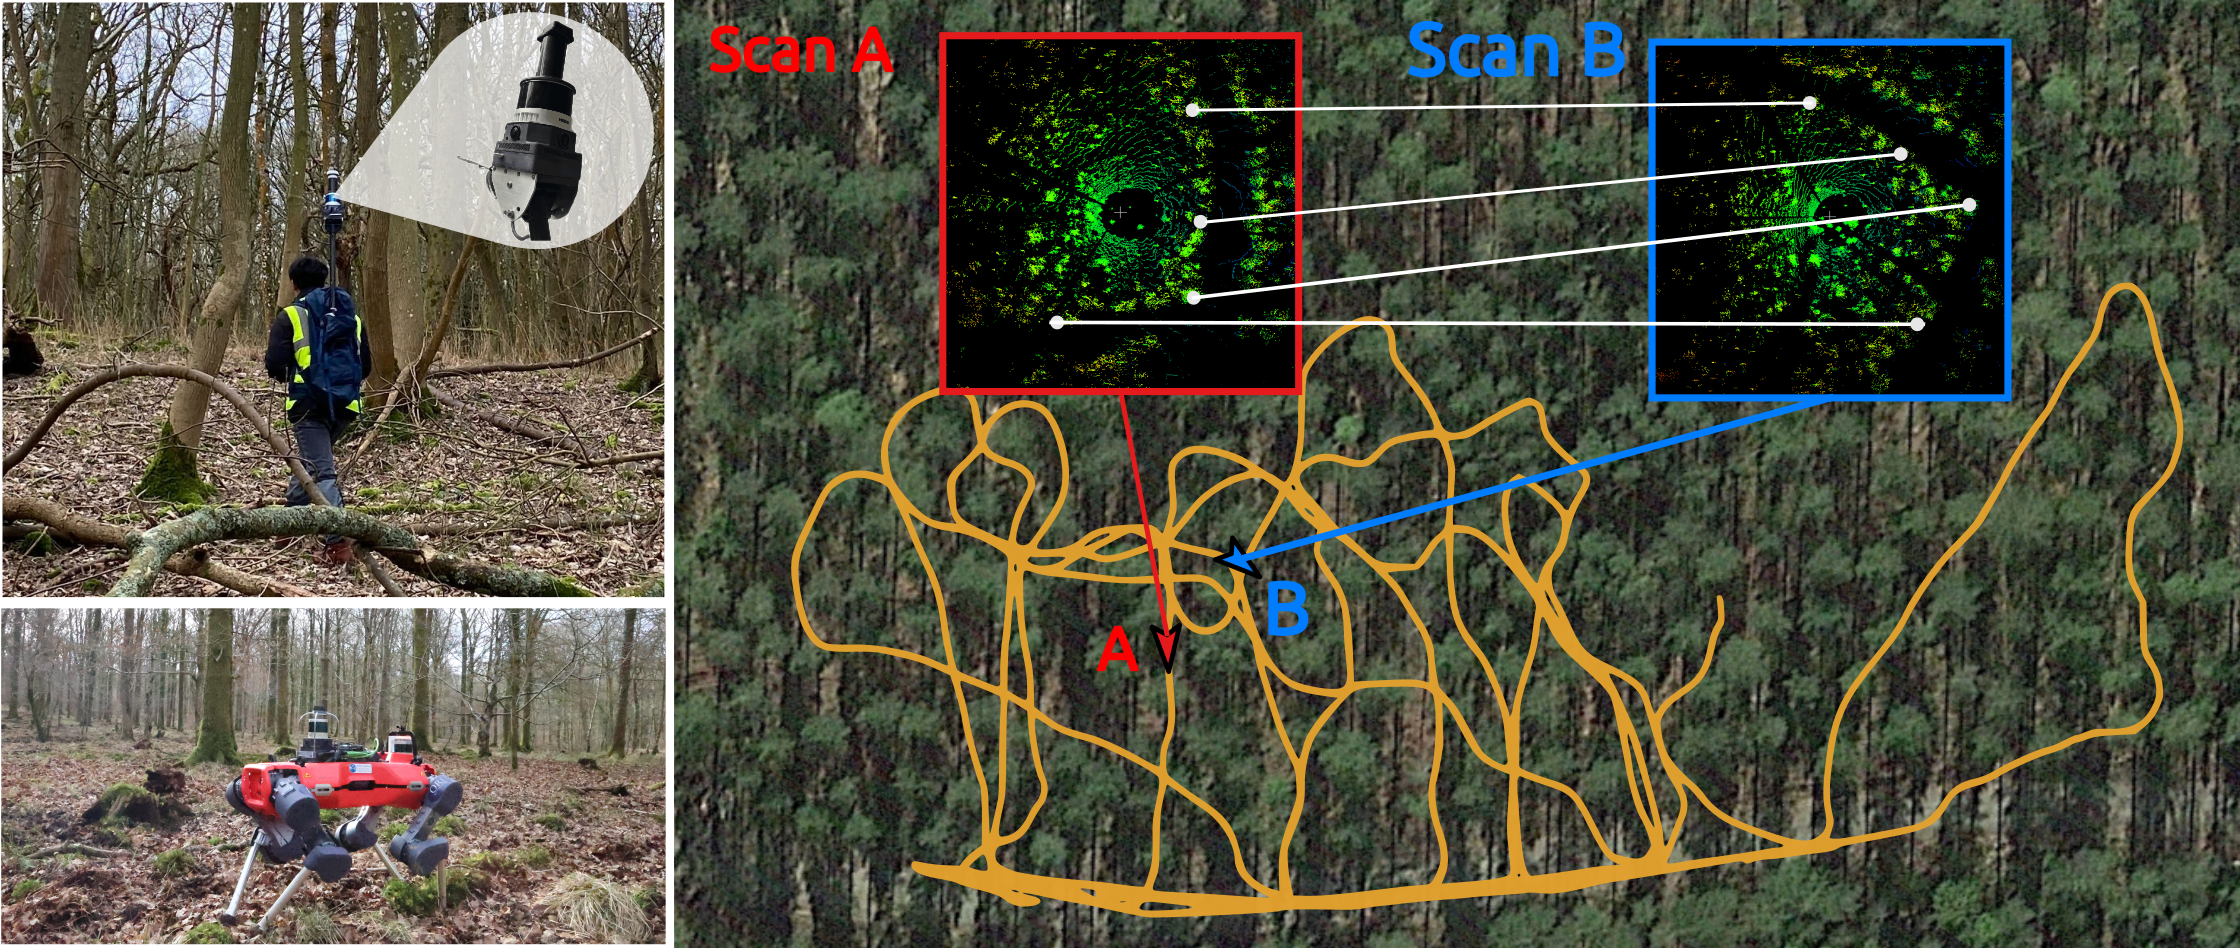
\includegraphics[width=\linewidth]{pics/header.png}
    \captionof{figure}{Place recognition in dense forest environments using a backpack-mounted LiDAR and legged robot equipped with LiDAR. Right: Illustration of loop closure detection within a deeply forested area, with offset distance of 9.2 meters and orientation of 56 degrees between the matched scans. White lines indicate some corresponding locations in the two point clouds (but no actual corresponces are used).
    }
    \label{fig:motivation}
\end{figure}

\section{Motivation}
Place recognition is an essential capability used to minimize the drift in the pose estimate produce by a Simultaneous Localization and Mapping (SLAM), as well as to re-localize in previously mapped areas. 
LiDAR-based place recognition systems have demonstrated robustness by effectively capturing scene structure while showing low susceptibility to visual changes, making them suitable for long-term navigation. 
Previous methods have primarily focused on the problem of autonomous driving in urban environments (characterised by long linear sequences), with their efficacy in natural settings much less tested.
%\mfallon{Wildplaces dataset is a counter example of this.} 
Recent ongoing applications in natural environments, including agriculture, environmental monitoring, conservation, and search and rescue, highlight the significance of extending research efforts beyond urban landscapes.

\section{Challenges in natural environments}
% Why natural environment 
Despite the advancements of LiDAR-based place recognition in urban areas, its application in unstructured natural environments like forests presents several notable challenges. 
Firstly, natural environments are irregular structures like trees, which not only lack fine structure but also undergo seasonal changes, affecting their shape and density over time. This complicates the creation of consistent geometric representations crucial for accurate place recognition.
Secondly, a limited field of view and occlusions of a LiDAR sensor pose a loss of information. In large-scale natural environment, LiDAR sensors often struggle to capture the complete vertical extent of the environment. 
This issue is particularly common in areas with tall, cluttered trees.  Undulating terrains and dense trees cause occlusions resulting in incomplete scans of a LiDAR sensor. 
Lastly, unique, undefined trajectories or paths when exploring dense forests pose another challenge: a place recognition capability of identifying its location not exctly at the same visited place but 'near by' location. 


%%%%%%%%%%%%%%%%%%%
%% WHICH PROBLEM
% Second, explain WHICH problem you are solving/address to solve: Compare WildPlace  
\section{Objectives}
Recently, the Wild-Places dataset \cite{knights2023icra} has been made available. In it a large-scale forest dataset was captured by hand-held spinning LiDAR, capturing seasonal changes within the forest. The dataset was used to evaluate different stete-of-the-art place recognition models in forest environments focusing on localization tasks along the access roads of a national park. The main outcome of their work was that learning-based descriptors such as Logg3dNet \cite{vidanapathirana2022icra} showed better performance compared to handcrafted methods such as ScanContext \cite{kim2018iros}. While the findings suggested that LiDAR-based methods could provide a solution for place-based localization in forest environments, it was not conclusive if the results transferred to dense forest areas, without the strong structural cues that access roads provide roads. Additionally we are also interested in testing the accuracy of precise 6DoF pose estimation for forestry or biodiversity monitoring applications.


%%%%%%%%%%%%%%%%%%%
%% HOW & WHAT
% Third, explain briefly how one can address the problem in general and mention 
% briefly what others/we before have done. Prepare the reader for your contribution that comes in the next section (and not here!).
%\mfallon{this paragraph should be a little literature review - NOT about what we did}
%\haedam{I changed the paragraph to be more about WildPlace}

% In this paper, we extend the evaluation of place recognition models to dense forest environments, employing various setups of LiDAR sensors. For instance, we consider scenarios involving legged robots or backpack-mounted LiDAR devices, which explore the forest in a more unstructured manner, without relying on defined access roads for detecting loop-closures.
% This extension enables for efficient forest mapping and surveying applications in scenarios including single-session and multi-session SLAM, as well as relocalization within a pre-existing map.

%%%%%%%%%%%%%%%%%%%
%% MAIN CONTRIBUTION & WHAT FOLLOWS FROM THAT
% Explain your contribution in one paragraph. This is a very important paragraph. 
% Always start that paragraph with: ``The main contribution of this paper is''
\section{Contributions}

In this work, we present an evaluation of place recognition models to dense forest environments. We employ different LiDAR sensors with sequences recorded with backpack-mounted devices or mobile robots, such as legged platforms, to perform a rigorous analysis of existing learning-based and handcrafted LiDAR place recognition systems. Further, we present a LiDAR-based SLAM system to assess the proposed loop-closure pairs and subsequently validate them through fine-registration in both online and offline modes. Finally, we demonstrate the approach being use for a purely relocalization task, wherein the system continuously localizes its position within a prior point cloud map made up of individual LiDAR scans.

% \mfallon{Note: alternatively you could simply localise in a single giant point cloud of the forest - if you knew the starting point - but that would not scale well. But it would work!}

%%%%%%%%%%%%%%%%%%%
%% OUR KEY CLAIMS (can be merged with the main contribution above if desired)
% Explicitly(!) state your claims in one (short) paragraph and make
% sure you pick them up again in the experiments and support every claim.

In summary, the contributions of this paper are:
\begin{itemize}

\item Evaluation of the performance of four LiDAR place recognition models, both handcrafted and learning-based, in dense forest environments.

\item Analyzis of loop-closure performance as a function of the relative distance and orientation between candidate loop pairs.

\item Demonstration of the best performing method in online/single-session and offline/multi-session SLAM modes, as well as in relocalization tasks for forest inspection in a prior environment map. 
% \mfallon{what about `Demonstration of the best performing method...' in these tasks}

\end{itemize}






% \section{Motivation}

% Legged robots have the potential to perform tasks that are extremely challenging or risky for humans, such as exploration of unknown locations or rescue operations. The recent \gls{darpa} SubT challenge (2018-2021) was a clear demonstration of the advantages of such platforms for exploration in urban and underground environments~\cite{Ackerman2022}. When the challenge started in 2018, 3 out of 11 teams were using legged robots for the competition; 3 years later almost every team relied on them as their core platforms~\cite{Chung2023}. Their versatility when negotiating different kinds of terrain compared to wheeled robots, as well as their increased payload capabilities compared to aerial ones offer a good balance for their deployment in the field.

% A key aspect of this success has been the impressive mobility skills achieved by the locomotion controllers developed by the research community over the last few years~\cite{Gangapurwala2020, Miki2022a, Kumar2021}, combined with the consolidation of commercial platforms such as the Boston Dynamics' Spot~\cite{BostonDynamics} and ANYbotics' ANYmal~\cite{Anybotics} quadrupeds, and humanoids such as the Agility Robotics' Digit~\cite{AgilityRobotics}. This offers an unprecedented scenario for their mass adoption in applications such as last-mile delivery, industrial inspection, monitoring, or rescue.

% The new locomotion controllers have unlocked new environments where legged robots can operate: not only warehouses with flat terrain but also industrial environments with complex staircases~\cite{BostonDynamics}, urban and disaster scenarios~\cite{Lee2020}, underground environments~\cite{Miki2022a}, as well as natural scenes such as foThe main objectives are to evaluate the performance of existing LiDAR-based place recognition models in dense forest environments.motivation/motivation.jpg}
% 	\caption{Autonomous deployments of legged robots using the contributions presented in this thesis. They include industrial environments, underground mines, public parks, and forests.}
% 	\label{fig:motivation}
% \end{figure}

% \section{Objective}
% The main objective of this thesis is to develop new navigation systems for legged robots. We define navigation as the problem of safely moving between two locations A and B while avoiding obstacles and other risky areas~\cite{Corke2011,Lynch2017,Ekstrom2018}. While the definition is concise, developing such capabilities for robotic systems is a complex problem that requires a strong coordination of perception, planning, and control methods.

% The second objective is then to develop the specific systems and methods that, when seamlessly integrated, enable legged robot navigation.

% Last, we aim to achieve navigation in challenging environments: spaces that can be dynamic, difficult to access by humans, or simply risky. Specific examples include  industrial facilities, mines, tunnels, or open natural scenes.

% %In this work we present three solutions for this purpose. They address localisation, scene understanding and local planning with legged platforms. These have been tested onboard, in closed-loop, demonstrating real-world navigation in environments such as structured industrial facilities, underground mines, and forests, .

% \section{Contributions}
% The main contribution of this thesis is the investigation, implementation, and field deployment of new navigation systems to expand the use of legged robots in challenging environments, as shown in \figref{fig:motivation}. The systems were designed to be simple but principled, exploiting fundamental ideas of optimisation methods as well as the constraints and advantages that legged robots present.

% The specific contributions of this work include:
% \begin{itemize}[leftmargin=*]
% 	\item An entropy-based approach for active camera selection that robustifies multi-camera localisation systems under transient scene changes.
% 	\item A local planning system that relies on local scene representations to achieve safe and reactive navigation.
% 	\item A framework for self-supervised online traversability learning that enables fast deployment in unknown environments.
% 	\item A mission planning system for autonomous forest inventory with legged robots.
% 	\item Hardware integration and deployment of these systems on legged platforms in industrial, underground, and natural environments.
% \end{itemize}



% \section{Thesis Outline}
% This thesis is presented in the \emph{integrated format} of the University of Oxford. Chapters 4-6 consist of peer-reviewed publications, each one accompanied by additional discussion as well as a Statement of Authorship declaring the author's contribution to each work. Chapter 7 is an original chapter describing a real-world application.

% The remainder of the thesis is structured as follows:
% \begin{itemize}[leftmargin=*]
% 	%\item \textbf{Chapter 1 -- Introduction:} The present chapter, summarising the objectives, contributions, and achievements.
% 	\item \textbf{Chapter 2 -- Background:} Presentation of the main definitions, theory, and methods used in the thesis.
% 	\item \textbf{Chapter 3 - Related Work:} Review of the relevant literature on robot navigation, with a particular focus on legged platforms.
% 	\item \textbf{Chapter 4 -- Multi-camera Visual Localisation:} An approach to reliably localising robots by actively choosing the \emph{most informative} camera during deployment.
% 	\item \textbf{Chapter 5 -- Reactive Local Planning:} How to navigate in challenging, narrow environments using a reactive local planning approach.
% 	\item \textbf{Chapter 6 -- Online Traversability Learning:} Overcoming the challenges of data collection and curation in traversability estimation via online self-supervised learning.
% 	\item \textbf{Chapter 7 -- Autonomous Forest Inventory:} Conceptualisation and field deployment of autonomous legged robots for forestry applications.
% 	\item \textbf{Chapter 8 -- Conclusion:} Discussion on the achievements and limitations of this work, lessons learned, and future directions for the field.
% \end{itemize}